\documentclass[11pt]{article}
\usepackage[
top    = 2.50cm,% presumably you don't want it to be 0pt as well?
bottom = 2.50cm,
left   = 2cm,
right  = 2cm,
marginparsep = 0pt,
marginparwidth=0pt,
]{geometry}

\usepackage{amssymb}
\usepackage{fancyhdr}
\usepackage{siunitx}
\usepackage{amsmath}
\usepackage{tikz}
\usepackage{caption}
\usepackage{pgfplots}
\usepackage{multicol}
\pagestyle{fancy}
\fancyhead[l]{Mechanics: Kinematics - Abridged edition}
\fancyhead[r]{Giorgio G.}

\begin{document}
	
\section{Graphs of motion: }
\subsection{Displacement-time graphs:}
\begin{multicols}{3}
	{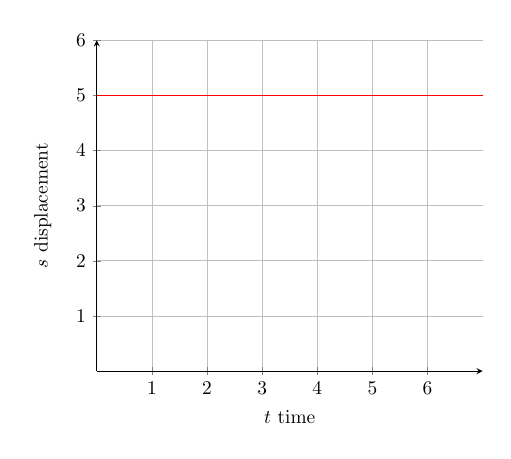
\begin{tikzpicture}[scale=0.7]
			\begin{axis}[
				x=1cm,y=1cm,
				axis lines=middle,
				ymajorgrids=true,
				xmajorgrids=true,
				xmin=0,
				xmax=7,
				ymin=0,
				x label style={at={(axis description cs:0.5,-0.1)},anchor=north},
				y label style={at={(axis description cs:-0.1,0.5)},rotate=90,anchor=south},
				xlabel=$t$ time,
				ylabel=$s$ displacement,
				ymax=6,
				xtick={0,1,...,6},
				ytick={0,1,...,6},]
			\end{axis}
			\draw[color=red,domain=0:7,samples=1000] plot ({\x},5);
		\end{tikzpicture}
	\captionof*{figure}{\qquad \qquad \qquad No velocity}}
	{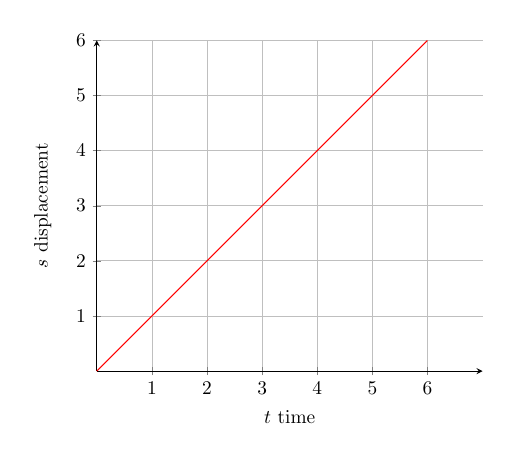
\begin{tikzpicture}[scale=0.7]
			\begin{axis}[
				x=1cm,y=1cm,
				axis lines=middle,
				ymajorgrids=true,
				xmajorgrids=true,
				xmin=0,
				xmax=7,
				ymin=0,
				x label style={at={(axis description cs:0.5,-0.1)},anchor=north},
				y label style={at={(axis description cs:-0.1,0.5)},rotate=90,anchor=south},
				xlabel=$t$ time,
				ylabel=$s$ displacement,
				ymax=6,
				xtick={0,1,...,6},
				ytick={0,1,...,6},]
			\end{axis}
			\draw[color=red,domain=0:6,samples=1000] plot ({\x},({\x});
		\end{tikzpicture}

	\captionof*{figure}{\qquad\qquad\qquad Velocity is constant}
	}

	{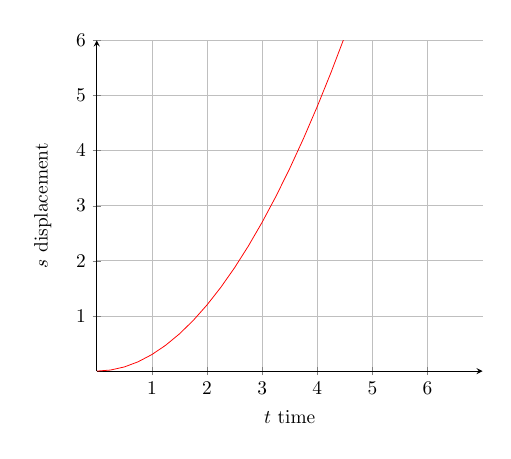
\begin{tikzpicture}[scale=0.7]
		\begin{axis}[
			x=1cm,y=1cm,
			axis lines=middle,
			ymajorgrids=true,
			xmajorgrids=true,
			xmin=0,
			xmax=7,
			ymin=0,
			x label style={at={(axis description cs:0.5,-0.1)},anchor=north},
			y label style={at={(axis description cs:-0.1,0.5)},rotate=90,anchor=south},
			xlabel=$t$ time,
			ylabel=$s$ displacement,
			ymax=6,
			xtick={0,1,...,6},
			ytick={0,1,...,6},]
			\addplot[color=red, domain=0:6]{0.3*x^2};
		\end{axis}
	\end{tikzpicture}
\captionof*{figure}{\qquad \qquad\qquad Velocity increasing}}
\end{multicols}

\subsection{Velocity-time graphs:  }
\begin{multicols}{3}
	{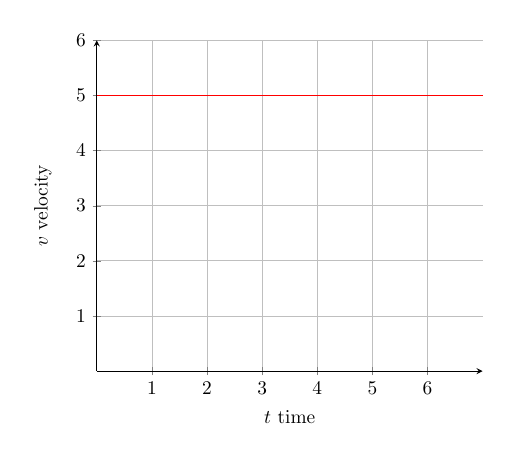
\begin{tikzpicture}[scale=0.7]
			\begin{axis}[
				x=1cm,y=1cm,
				axis lines=middle,
				ymajorgrids=true,
				xmajorgrids=true,
				xmin=0,
				xmax=7,
				ymin=0,
				x label style={at={(axis description cs:0.5,-0.1)},anchor=north},
				y label style={at={(axis description cs:-0.1,0.5)},rotate=90,anchor=south},
				xlabel=$t$ time,
				ylabel=$v$ velocity,
				ymax=6,
				xtick={0,1,...,6},
				ytick={0,1,...,6},]
			\end{axis}
			\draw[color=red,domain=0:7,samples=1000] plot ({\x},5);
		\end{tikzpicture}
		\captionof*{figure}{\qquad \qquad \qquad Constant velocity}}
	{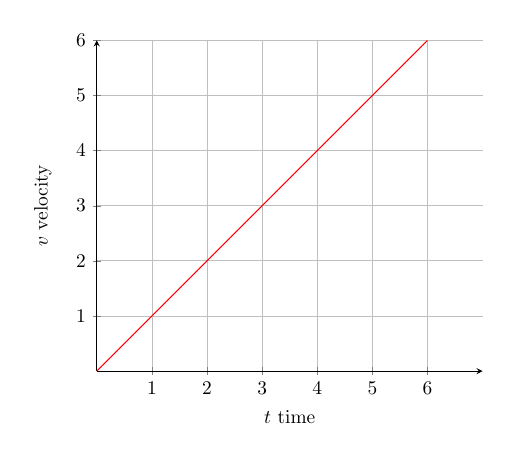
\begin{tikzpicture}[scale=0.7]
			\begin{axis}[
				x=1cm,y=1cm,
				axis lines=middle,
				ymajorgrids=true,
				xmajorgrids=true,
				xmin=0,
				xmax=7,
				ymin=0,
				x label style={at={(axis description cs:0.5,-0.1)},anchor=north},
				y label style={at={(axis description cs:-0.1,0.5)},rotate=90,anchor=south},
				xlabel=$t$ time,
				ylabel=$v$ velocity,
				ymax=6,
				xtick={0,1,...,6},
				ytick={0,1,...,6},]
			\end{axis}
			\draw[color=red,domain=0:6,samples=1000] plot ({\x},({\x});
		\end{tikzpicture}
		
		\captionof*{figure}{\qquad\qquad \quad Constant acceleration}
	}
	
	{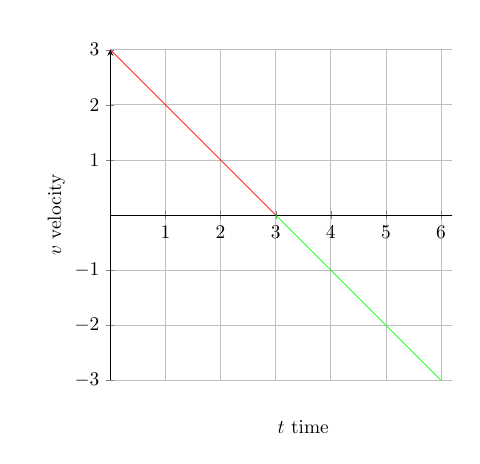
\begin{tikzpicture}[scale=0.7]
				\clip(-1.5,-1) rectangle (6.2,6.4);
			\begin{axis}[
				x=1cm,y=1cm,
				axis lines=middle,
				ymajorgrids=true,
				xmajorgrids=true,
				xmin=0,
				xmax=7,
				ymin=-3,
				x label style={at={(axis description cs:0.5,-0.1)},anchor=north},
				y label style={at={(axis description cs:-0.1,0.5)},rotate=90,anchor=south},
				xlabel=$t$ time,
				ylabel=$v$ velocity,
				ymax=3,
				xtick={0,1,...,6},
				ytick={-3,-2,...,3},]
				\addplot[color=red, domain=0:3]{-x+3};
				\addplot[color=green, domain=3:6]{-x+3};
				\end{axis}
		\end{tikzpicture}
		\captionof*{figure}{\qquad \quad \space \textcolor{red}{Deceleration}, \textcolor{green}{acceleration}}}
\end{multicols}
\section{Projectiles: }
\begin{multicols}{2}
	\begin{center}
		\underline{\textbf{Vertically}}
	\end{center}
\begin{equation}
	t=\sqrt{\frac{2s}{a}}\tag{\si{\second}}
\end{equation}
\begin{center}
	Where $t$ is the object's \textbf{air-time}, $s$ its \textbf{vertical displacement} from the ground, and $a$ the \textbf{acceleration} due to gravity.
\end{center}

\begin{center}
	\underline{\textbf{Horizontally}}
\end{center}

\begin{equation}
	s=ut\tag{\si{\meter}}
\end{equation}
\begin{center}
	Where $s$ is the object's \textbf{horizontal range}, $t$ its \textbf{air-time} previously found and $u$ its initial \textbf{push velocity}.
\end{center}
\end{multicols}
 
\end{document}